\documentclass[tikz,border=8pt]{standalone}
% Shared look for every TikZ diagram. Load with \input{../../tools/tikz-style.tex}
\usepackage[T1]{fontenc}
\usepackage{lmodern}
\renewcommand{\sfdefault}{lmr}  % diagrams use the same serif as the text
\usetikzlibrary{arrows.meta, positioning, shapes.geometric, calc, fit, backgrounds}
\definecolor{cblue}{HTML}{4C78A8}
\definecolor{corange}{HTML}{F58518}
\definecolor{cgreen}{HTML}{54A24B}
\definecolor{cred}{HTML}{E45756}
\definecolor{cpurple}{HTML}{B279A2}
\definecolor{cgrey}{HTML}{6B6B6B}
\tikzset{
  every picture/.style={font=\sffamily, line width=1.2pt},
  box/.style={draw=#1, fill=#1!12, rounded corners=4pt, align=center, inner sep=7pt, minimum height=1.1cm},
  box/.default=cgrey,
  arrow/.style={-{Stealth[length=3mm]}, draw=cgrey, line width=1.4pt},
  title/.style={font=\sffamily\bfseries\Large},
  note/.style={font=\sffamily\small, text=cgrey, align=center},
}
\AtBeginDocument{\hyphenpenalty=10000 \exhyphenpenalty=10000}

\begin{document}
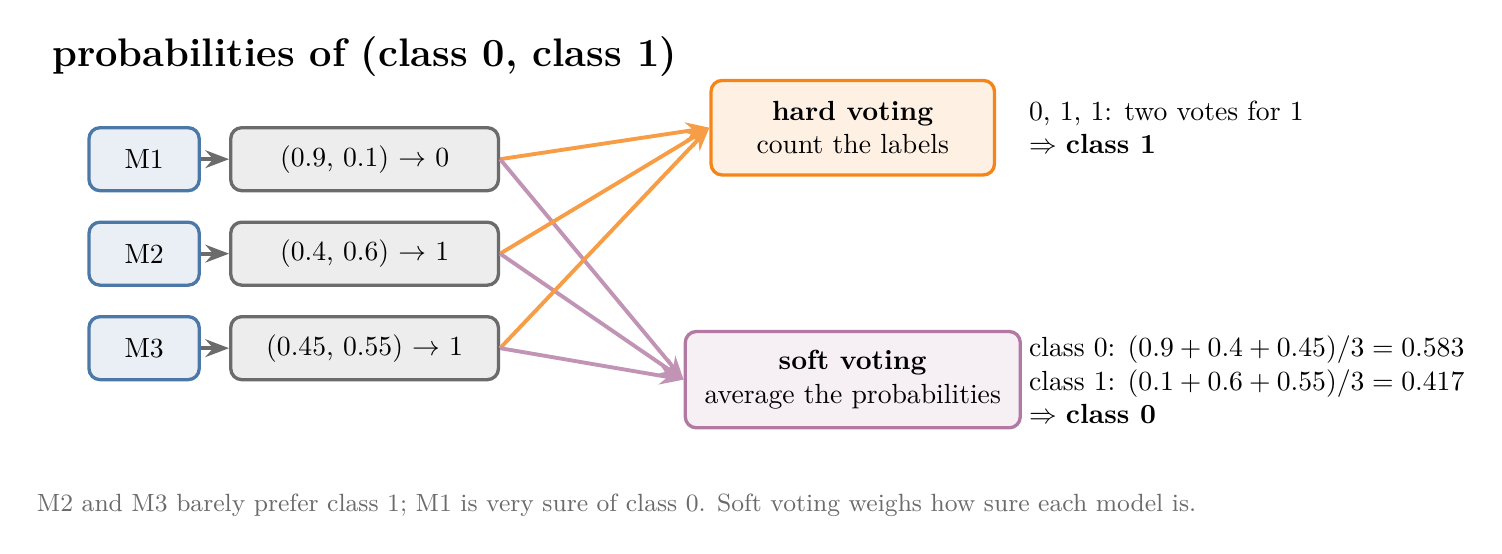
\begin{tikzpicture}[
  m/.style={box=cblue, minimum width=1.4cm, minimum height=0.8cm, inner sep=3pt},
  pr/.style={box=cgrey, minimum width=3.4cm, minimum height=0.8cm, inner sep=3pt},
  hv/.style={box=corange, minimum width=3.6cm, minimum height=1.2cm},
  sv/.style={box=cpurple, minimum width=3.6cm, minimum height=1.2cm}]
  \node[title] at (2.8,1.3) {probabilities of (class 0, class 1)};
  \node[m] (m1) at (0,0) {M1};      \node[pr] (p1) at (2.8,0) {(0.9, 0.1) $\rightarrow$ 0};
  \node[m] (m2) at (0,-1.2) {M2};   \node[pr] (p2) at (2.8,-1.2) {(0.4, 0.6) $\rightarrow$ 1};
  \node[m] (m3) at (0,-2.4) {M3};   \node[pr] (p3) at (2.8,-2.4) {(0.45, 0.55) $\rightarrow$ 1};
  \foreach \i in {1,2,3} \draw[arrow] (m\i) -- (p\i);
  \node[hv] (h) at (9.0,0.4) {\textbf{hard voting}\\count the labels};
  \node[sv] (s) at (9.0,-2.8) {\textbf{soft voting}\\average the probabilities};
  \foreach \i in {1,2,3} {\draw[arrow, draw=corange!80] (p\i.east) -- (h.west); \draw[arrow, draw=cpurple!80] (p\i.east) -- (s.west);}
  \node[anchor=west, align=left] at (11.1,0.4) {0, 1, 1: two votes for 1\\$\Rightarrow$ \textbf{class 1}};
  \node[anchor=west, align=left] at (11.1,-2.8) {class 0: $(0.9 + 0.4 + 0.45)/3 = 0.583$\\class 1: $(0.1 + 0.6 + 0.55)/3 = 0.417$\\$\Rightarrow$ \textbf{class 0}};
  \node[note] at (6,-4.4) {M2 and M3 barely prefer class 1; M1 is very sure of class 0. Soft voting weighs how sure each model is.};
\end{tikzpicture}
\end{document}
